\documentclass[twoside]{book}

% Packages required by doxygen
\usepackage{fixltx2e}
\usepackage{calc}
\usepackage{doxygen}
\usepackage[export]{adjustbox} % also loads graphicx
\usepackage{graphicx}
\usepackage[utf8]{inputenc}
\usepackage{makeidx}
\usepackage{multicol}
\usepackage{multirow}
\PassOptionsToPackage{warn}{textcomp}
\usepackage{textcomp}
\usepackage[nointegrals]{wasysym}
\usepackage[table]{xcolor}

% Font selection
\usepackage[T1]{fontenc}
\usepackage[scaled=.90]{helvet}
\usepackage{courier}
\usepackage{amssymb}
\usepackage{sectsty}
\renewcommand{\familydefault}{\sfdefault}
\allsectionsfont{%
  \fontseries{bc}\selectfont%
  \color{darkgray}%
}
\renewcommand{\DoxyLabelFont}{%
  \fontseries{bc}\selectfont%
  \color{darkgray}%
}
\newcommand{\+}{\discretionary{\mbox{\scriptsize$\hookleftarrow$}}{}{}}

% Page & text layout
\usepackage{geometry}
\geometry{%
  a4paper,%
  top=2.5cm,%
  bottom=2.5cm,%
  left=2.5cm,%
  right=2.5cm%
}
\tolerance=750
\hfuzz=15pt
\hbadness=750
\setlength{\emergencystretch}{15pt}
\setlength{\parindent}{0cm}
\setlength{\parskip}{3ex plus 2ex minus 2ex}
\makeatletter
\renewcommand{\paragraph}{%
  \@startsection{paragraph}{4}{0ex}{-1.0ex}{1.0ex}{%
    \normalfont\normalsize\bfseries\SS@parafont%
  }%
}
\renewcommand{\subparagraph}{%
  \@startsection{subparagraph}{5}{0ex}{-1.0ex}{1.0ex}{%
    \normalfont\normalsize\bfseries\SS@subparafont%
  }%
}
\makeatother

% Headers & footers
\usepackage{fancyhdr}
\pagestyle{fancyplain}
\fancyhead[LE]{\fancyplain{}{\bfseries\thepage}}
\fancyhead[CE]{\fancyplain{}{}}
\fancyhead[RE]{\fancyplain{}{\bfseries\leftmark}}
\fancyhead[LO]{\fancyplain{}{\bfseries\rightmark}}
\fancyhead[CO]{\fancyplain{}{}}
\fancyhead[RO]{\fancyplain{}{\bfseries\thepage}}
\fancyfoot[LE]{\fancyplain{}{}}
\fancyfoot[CE]{\fancyplain{}{}}
\fancyfoot[RE]{\fancyplain{}{\bfseries\scriptsize Generated by Doxygen }}
\fancyfoot[LO]{\fancyplain{}{\bfseries\scriptsize Generated by Doxygen }}
\fancyfoot[CO]{\fancyplain{}{}}
\fancyfoot[RO]{\fancyplain{}{}}
\renewcommand{\footrulewidth}{0.4pt}
\renewcommand{\chaptermark}[1]{%
  \markboth{#1}{}%
}
\renewcommand{\sectionmark}[1]{%
  \markright{\thesection\ #1}%
}

% Indices & bibliography
\usepackage{natbib}
\usepackage[titles]{tocloft}
\setcounter{tocdepth}{3}
\setcounter{secnumdepth}{5}
\makeindex

% Hyperlinks (required, but should be loaded last)
\usepackage{ifpdf}
\ifpdf
  \usepackage[pdftex,pagebackref=true]{hyperref}
\else
  \usepackage[ps2pdf,pagebackref=true]{hyperref}
\fi
\hypersetup{%
  colorlinks=true,%
  linkcolor=blue,%
  citecolor=blue,%
  unicode%
}

% Custom commands
\newcommand{\clearemptydoublepage}{%
  \newpage{\pagestyle{empty}\cleardoublepage}%
}

\usepackage{caption}
\captionsetup{labelsep=space,justification=centering,font={bf},singlelinecheck=off,skip=4pt,position=top}

%===== C O N T E N T S =====

\begin{document}

% Titlepage & ToC
\hypersetup{pageanchor=false,
             bookmarksnumbered=true,
             pdfencoding=unicode
            }
\pagenumbering{alph}
\begin{titlepage}
\vspace*{7cm}
\begin{center}%
{\Large My Project \\[1ex]\large 1 }\\
\vspace*{1cm}
{\large Generated by Doxygen 1.8.13}\\
\end{center}
\end{titlepage}
\clearemptydoublepage
\pagenumbering{roman}
\tableofcontents
\clearemptydoublepage
\pagenumbering{arabic}
\hypersetup{pageanchor=true}

%--- Begin generated contents ---
\chapter{File Index}
\section{File List}
Here is a list of all files with brief descriptions\+:\begin{DoxyCompactList}
\item\contentsline{section}{/home/kavya/\+Desktop/csn261\+\_\+lab\+\_\+assignment1/q1/code/\hyperlink{q1_8c}{q1.\+c} }{\pageref{q1_8c}}{}
\end{DoxyCompactList}

\chapter{File Documentation}
\hypertarget{q3_8cpp}{}\section{code/q3.cpp File Reference}
\label{q3_8cpp}\index{code/q3.\+cpp@{code/q3.\+cpp}}


this program implements Bentley-\/\+Ottmann Algorithm to find all intersection of n given lines and also find linear fit.  


{\ttfamily \#include $<$iostream$>$}\newline
{\ttfamily \#include $<$vector$>$}\newline
{\ttfamily \#include $<$map$>$}\newline
{\ttfamily \#include $<$cmath$>$}\newline
Include dependency graph for q3.\+cpp\+:
\nopagebreak
\begin{figure}[H]
\begin{center}
\leavevmode
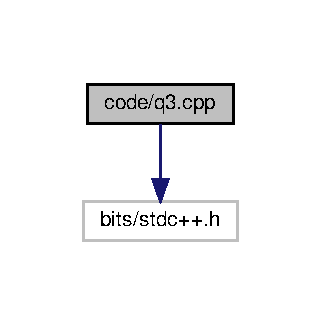
\includegraphics[width=312pt]{q3_8cpp__incl}
\end{center}
\end{figure}
\subsection*{Classes}
\begin{DoxyCompactItemize}
\item 
struct \hyperlink{struct_point}{Point}
\begin{DoxyCompactList}\small\item\em this is the struct of \hyperlink{struct_point}{Point} which represent any point. \end{DoxyCompactList}\item 
struct \hyperlink{struct_line}{Line}
\begin{DoxyCompactList}\small\item\em this is struct which represent any line segment. \end{DoxyCompactList}\item 
class \hyperlink{classevent__less}{event\+\_\+less}
\begin{DoxyCompactList}\small\item\em this is event-\/less class which contain operator function which define some operation on the line. \end{DoxyCompactList}\end{DoxyCompactItemize}
\subsection*{Functions}
\begin{DoxyCompactItemize}
\item 
pair$<$ bool, \hyperlink{struct_point}{Point} $>$ \hyperlink{q3_8cpp_a9ba35f40883641283fb96b6ad2b384ee}{intersect} (const \hyperlink{struct_line}{Line} \&a, const \hyperlink{struct_line}{Line} \&b, bool print)
\begin{DoxyCompactList}\small\item\em this function make some possible pair. \end{DoxyCompactList}\item 
void \hyperlink{q3_8cpp_a6aa32d408e7d87f7c058294626b6b9b0}{intersect} (int a, int b, const \hyperlink{struct_point}{Point} \&I, vector$<$ \hyperlink{struct_line}{Line} $>$ \&lines, multimap$<$ \hyperlink{struct_point}{Point}, int $>$ \&sweep, multimap$<$ pair$<$ double, int $>$, int, \hyperlink{classevent__less}{event\+\_\+less} $>$ \&events, bool print)
\item 
void \hyperlink{q3_8cpp_a2d57adc002542eee576c8c1442871b4d}{intersect} (vector$<$ \hyperlink{struct_line}{Line} $>$ \&lines, vector$<$ \hyperlink{struct_point}{Point} $>$ \&intersections, bool print)
\begin{DoxyCompactList}\small\item\em this function find all possible intersection of the n given lines. \end{DoxyCompactList}\item 
void \hyperlink{q3_8cpp_afeefc4b0befb61aa570a24d552271099}{linearfitline} (double x\mbox{[}$\,$\mbox{]}, double y\mbox{[}$\,$\mbox{]}, int n)
\begin{DoxyCompactList}\small\item\em this fucntion find linearfit of M found intersection points using least square method. \end{DoxyCompactList}\item 
int \hyperlink{q3_8cpp_ae66f6b31b5ad750f1fe042a706a4e3d4}{main} ()
\begin{DoxyCompactList}\small\item\em this is the main function. \end{DoxyCompactList}\end{DoxyCompactItemize}
\subsection*{Variables}
\begin{DoxyCompactItemize}
\item 
int \hyperlink{q3_8cpp_adc735e446799084e3d27da58cf5807c3}{seg\+\_\+start} =0
\item 
int \hyperlink{q3_8cpp_a4311f4976e51399caed297d2cad3bfd3}{seg\+\_\+end} =1
\end{DoxyCompactItemize}


\subsection{Detailed Description}
this program implements Bentley-\/\+Ottmann Algorithm to find all intersection of n given lines and also find linear fit. 

Kavya Barnwal \begin{DoxyDate}{Date}
2019-\/10-\/08 
\end{DoxyDate}


\subsection{Function Documentation}
\mbox{\Hypertarget{q3_8cpp_a9ba35f40883641283fb96b6ad2b384ee}\label{q3_8cpp_a9ba35f40883641283fb96b6ad2b384ee}} 
\index{q3.\+cpp@{q3.\+cpp}!intersect@{intersect}}
\index{intersect@{intersect}!q3.\+cpp@{q3.\+cpp}}
\subsubsection{\texorpdfstring{intersect()}{intersect()}\hspace{0.1cm}{\footnotesize\ttfamily [1/3]}}
{\footnotesize\ttfamily pair$<$bool, \hyperlink{struct_point}{Point}$>$ intersect (\begin{DoxyParamCaption}\item[{const \hyperlink{struct_line}{Line} \&}]{a,  }\item[{const \hyperlink{struct_line}{Line} \&}]{b,  }\item[{bool}]{print }\end{DoxyParamCaption})}



this function make some possible pair. 


\begin{DoxyParams}{Parameters}
{\em a} & \\
\hline
{\em b} & \\
\hline
{\em print} & \\
\hline
\end{DoxyParams}
\begin{DoxyReturn}{Returns}
pair$<$bool, Point$>$ 
\end{DoxyReturn}


Definition at line 81 of file q3.\+cpp.

\mbox{\Hypertarget{q3_8cpp_a6aa32d408e7d87f7c058294626b6b9b0}\label{q3_8cpp_a6aa32d408e7d87f7c058294626b6b9b0}} 
\index{q3.\+cpp@{q3.\+cpp}!intersect@{intersect}}
\index{intersect@{intersect}!q3.\+cpp@{q3.\+cpp}}
\subsubsection{\texorpdfstring{intersect()}{intersect()}\hspace{0.1cm}{\footnotesize\ttfamily [2/3]}}
{\footnotesize\ttfamily void intersect (\begin{DoxyParamCaption}\item[{int}]{a,  }\item[{int}]{b,  }\item[{const \hyperlink{struct_point}{Point} \&}]{I,  }\item[{vector$<$ \hyperlink{struct_line}{Line} $>$ \&}]{lines,  }\item[{multimap$<$ \hyperlink{struct_point}{Point}, int $>$ \&}]{sweep,  }\item[{multimap$<$ pair$<$ double, int $>$, int, \hyperlink{classevent__less}{event\+\_\+less} $>$ \&}]{events,  }\item[{bool}]{print }\end{DoxyParamCaption})}



Definition at line 117 of file q3.\+cpp.

\mbox{\Hypertarget{q3_8cpp_a2d57adc002542eee576c8c1442871b4d}\label{q3_8cpp_a2d57adc002542eee576c8c1442871b4d}} 
\index{q3.\+cpp@{q3.\+cpp}!intersect@{intersect}}
\index{intersect@{intersect}!q3.\+cpp@{q3.\+cpp}}
\subsubsection{\texorpdfstring{intersect()}{intersect()}\hspace{0.1cm}{\footnotesize\ttfamily [3/3]}}
{\footnotesize\ttfamily void intersect (\begin{DoxyParamCaption}\item[{vector$<$ \hyperlink{struct_line}{Line} $>$ \&}]{lines,  }\item[{vector$<$ \hyperlink{struct_point}{Point} $>$ \&}]{intersections,  }\item[{bool}]{print }\end{DoxyParamCaption})}



this function find all possible intersection of the n given lines. 


\begin{DoxyParams}{Parameters}
{\em lines} & \\
\hline
{\em intersections} & \\
\hline
{\em print} & \\
\hline
\end{DoxyParams}


Definition at line 164 of file q3.\+cpp.

\mbox{\Hypertarget{q3_8cpp_afeefc4b0befb61aa570a24d552271099}\label{q3_8cpp_afeefc4b0befb61aa570a24d552271099}} 
\index{q3.\+cpp@{q3.\+cpp}!linearfitline@{linearfitline}}
\index{linearfitline@{linearfitline}!q3.\+cpp@{q3.\+cpp}}
\subsubsection{\texorpdfstring{linearfitline()}{linearfitline()}}
{\footnotesize\ttfamily void linearfitline (\begin{DoxyParamCaption}\item[{double}]{x\mbox{[}$\,$\mbox{]},  }\item[{double}]{y\mbox{[}$\,$\mbox{]},  }\item[{int}]{n }\end{DoxyParamCaption})}



this fucntion find linearfit of M found intersection points using least square method. 


\begin{DoxyParams}{Parameters}
{\em x} & \\
\hline
{\em y} & \\
\hline
{\em n} & \\
\hline
\end{DoxyParams}


Definition at line 293 of file q3.\+cpp.

\mbox{\Hypertarget{q3_8cpp_ae66f6b31b5ad750f1fe042a706a4e3d4}\label{q3_8cpp_ae66f6b31b5ad750f1fe042a706a4e3d4}} 
\index{q3.\+cpp@{q3.\+cpp}!main@{main}}
\index{main@{main}!q3.\+cpp@{q3.\+cpp}}
\subsubsection{\texorpdfstring{main()}{main()}}
{\footnotesize\ttfamily int main (\begin{DoxyParamCaption}{ }\end{DoxyParamCaption})}



this is the main function. 

\begin{DoxyReturn}{Returns}
int 
\end{DoxyReturn}


Definition at line 314 of file q3.\+cpp.



\subsection{Variable Documentation}
\mbox{\Hypertarget{q3_8cpp_a4311f4976e51399caed297d2cad3bfd3}\label{q3_8cpp_a4311f4976e51399caed297d2cad3bfd3}} 
\index{q3.\+cpp@{q3.\+cpp}!seg\+\_\+end@{seg\+\_\+end}}
\index{seg\+\_\+end@{seg\+\_\+end}!q3.\+cpp@{q3.\+cpp}}
\subsubsection{\texorpdfstring{seg\+\_\+end}{seg\_end}}
{\footnotesize\ttfamily int seg\+\_\+end =1}



Definition at line 13 of file q3.\+cpp.

\mbox{\Hypertarget{q3_8cpp_adc735e446799084e3d27da58cf5807c3}\label{q3_8cpp_adc735e446799084e3d27da58cf5807c3}} 
\index{q3.\+cpp@{q3.\+cpp}!seg\+\_\+start@{seg\+\_\+start}}
\index{seg\+\_\+start@{seg\+\_\+start}!q3.\+cpp@{q3.\+cpp}}
\subsubsection{\texorpdfstring{seg\+\_\+start}{seg\_start}}
{\footnotesize\ttfamily int seg\+\_\+start =0}



Definition at line 13 of file q3.\+cpp.


%--- End generated contents ---

% Index
\backmatter
\newpage
\phantomsection
\clearemptydoublepage
\addcontentsline{toc}{chapter}{Index}
\printindex

\end{document}
